\documentclass{article}
\usepackage[utf8]{inputenc}
% \usepackage[russian]{babel}
\usepackage[a4paper, top=0.7in, left=0.5in, right=0.5in, bottom=0.6in, twocolumn]{geometry}
\usepackage{lastpage}
\usepackage{fancyhdr}
\usepackage{tikz}
\usepackage{pgfplots}
\usepackage{amssymb}
\usepackage{minted}
\usepackage{pdfpages}

\setcounter{secnumdepth}{5}
\setcounter{tocdepth}{5}
\pgfkeys{/pgf/number format/.cd,1000 sep={\,}}

\pagestyle{fancy}
\fancyhf{}
\lhead{ITMO University 1: Standard deviation (Budin, Kirillov, Sayutin)}
\rhead{Page \thepage\ of \pageref{LastPage}}
\lfoot{Generated \today}

\renewcommand{\footrulewidth}{0.4pt}
\setlength{\columnseprule}{0.4pt}

\begin{document}
\onecolumn
\tableofcontents

\twocolumn
\newpage

\section{Some useful things}
\inputminted[mathescape, breaklines, breakafter=(, tabsize=2, frame=lines, showtabs, tab=|\ , tabcolor=lightgray]{java}{./basic/Template.java}
\inputminted[mathescape, breaklines, breakafter=(, tabsize=2, frame=lines, showtabs, tab=|\ , tabcolor=lightgray]{c++}{./basic/io.cpp}
\inputminted[mathescape, breaklines, breakafter=(, tabsize=2, frame=lines, showtabs, tab=|\ , tabcolor=lightgray]{c++}{./basic/opt.cpp}
\inputminted[mathescape, breaklines, breakafter=(, tabsize=2, frame=lines, showtabs, tab=|\ , tabcolor=lightgray]{c++}{./basic/useful.cpp}
\section{Data structures}
\subsection{Hash table}
\inputminted[mathescape, breaklines, breakafter=(, tabsize=2, frame=lines, showtabs, tab=|\ , tabcolor=lightgray]{c++}{./data-structures/hash-table/hash-table.cpp}
\section{Geometry}
\subsection{Common tangents of two circles}
\inputminted[mathescape, breaklines, breakafter=(, tabsize=2, frame=lines, showtabs, tab=|\ , tabcolor=lightgray]{c++}{./geometry/common-tangents/common-tangents.cpp}
\subsection{Convex hull 3D in $O(n ^ 2)$}
\inputminted[mathescape, breaklines, breakafter=(, tabsize=2, frame=lines, showtabs, tab=|\ , tabcolor=lightgray]{c++}{./geometry/convex-hull-3d/convex-hull-3d.cpp}
\subsection{Dynamic convex hull trick}
\inputminted[mathescape, breaklines, breakafter=(, tabsize=2, frame=lines, showtabs, tab=|\ , tabcolor=lightgray]{c++}{./geometry/convex-hull-trick/convex-hull-trick.cpp}
\subsection{Minimal covering disk}
\inputminted[mathescape, breaklines, breakafter=(, tabsize=2, frame=lines, showtabs, tab=|\ , tabcolor=lightgray]{c++}{./geometry/min-disk/min-disk.cpp}
\subsection{Draw svg pictures}
\inputminted[mathescape, breaklines, breakafter=(, tabsize=2, frame=lines, showtabs, tab=|\ , tabcolor=lightgray]{c++}{./geometry/svg-draw/svg-draw.cpp}
\section{Graphs}
\subsection{2-Chinese algorithm}
\inputminted[mathescape, breaklines, breakafter=(, tabsize=2, frame=lines, showtabs, tab=|\ , tabcolor=lightgray]{c++}{./graphs/2-chinese/2-chinese.cpp}
\subsection{Dominator tree}
\inputminted[mathescape, breaklines, breakafter=(, tabsize=2, frame=lines, showtabs, tab=|\ , tabcolor=lightgray]{c++}{./graphs/dominator-tree/dominator-tree.cpp}
\subsection{General matching}
\inputminted[mathescape, breaklines, breakafter=(, tabsize=2, frame=lines, showtabs, tab=|\ , tabcolor=lightgray]{c++}{./graphs/general-matching/general-matching.cpp}
\subsection{Hungarian algorithm}
\inputminted[mathescape, breaklines, breakafter=(, tabsize=2, frame=lines, showtabs, tab=|\ , tabcolor=lightgray]{c++}{./graphs/hungarian-algorithm/hungarian-algorithm.cpp}
\subsection{Link-Cut Tree}
\inputminted[mathescape, breaklines, breakafter=(, tabsize=2, frame=lines, showtabs, tab=|\ , tabcolor=lightgray]{c++}{./graphs/link-cut-tree/link-cut-tree.cpp}
\subsection{Smith algorithm (Game on cyclic graph)}
\inputminted[mathescape, breaklines, breakafter=(, tabsize=2, frame=lines, showtabs, tab=|\ , tabcolor=lightgray]{c++}{./graphs/smith/smith.cpp}
\subsection{Stoer-Vagner algorithm (Global min-cut)}
\inputminted[mathescape, breaklines, breakafter=(, tabsize=2, frame=lines, showtabs, tab=|\ , tabcolor=lightgray]{c++}{./graphs/stoer-vagner/stoer-vagner.cpp}
\section{Matroids}
\subsection{Matroids intersection}
\inputminted[mathescape, breaklines, breakafter=(, tabsize=2, frame=lines, showtabs, tab=|\ , tabcolor=lightgray]{c++}{./matroids/matroids-intersection/matroids-intersection.cpp}
\section{Numeric}
\inputminted[mathescape, breaklines, breakafter=(, tabsize=2, frame=lines, showtabs, tab=|\ , tabcolor=lightgray]{c++}{./numeric/mod-ineq-first-sol.cpp}
\subsection{Berlekamp-Massey Algorithm}
\inputminted[mathescape, breaklines, breakafter=(, tabsize=2, frame=lines, showtabs, tab=|\ , tabcolor=lightgray]{c++}{./numeric/berlekamp/berlekamp.cpp}
\subsection{Chinese remainder theorem}
\inputminted[mathescape, breaklines, breakafter=(, tabsize=2, frame=lines, showtabs, tab=|\ , tabcolor=lightgray]{c++}{./numeric/chinese-remainder-theorem/chinese-remainder-theorem.cpp}
\subsection{Miller–Rabin primality test}
\inputminted[mathescape, breaklines, breakafter=(, tabsize=2, frame=lines, showtabs, tab=|\ , tabcolor=lightgray]{c++}{./numeric/miller-rabin/miller-rabin.cpp}
\subsection{Multiplication by modulo}
\inputminted[mathescape, breaklines, breakafter=(, tabsize=2, frame=lines, showtabs, tab=|\ , tabcolor=lightgray]{c++}{./numeric/mult-by-mod/mult-by-mod.cpp}
\subsection{Numerical integration}
\inputminted[mathescape, breaklines, breakafter=(, tabsize=2, frame=lines, showtabs, tab=|\ , tabcolor=lightgray]{c++}{./numeric/numerical-integration/numerical-integration.cpp}
\subsection{Pollard's rho algorithm}
\inputminted[mathescape, breaklines, breakafter=(, tabsize=2, frame=lines, showtabs, tab=|\ , tabcolor=lightgray]{c++}{./numeric/pollard/pollard.cpp}
\subsection{Polynom division and inversion}
\inputminted[mathescape, breaklines, breakafter=(, tabsize=2, frame=lines, showtabs, tab=|\ , tabcolor=lightgray]{c++}{./numeric/polynom-division/polynom-division.cpp}
\subsection{Simplex method}
\inputminted[mathescape, breaklines, breakafter=(, tabsize=2, frame=lines, showtabs, tab=|\ , tabcolor=lightgray]{c++}{./numeric/simplex/simplex.cpp}
\section{Strings}
\subsection{Duval algorithm (Lyndon factorization)}
\inputminted[mathescape, breaklines, breakafter=(, tabsize=2, frame=lines, showtabs, tab=|\ , tabcolor=lightgray]{c++}{./strings/duval/duval.cpp}
\subsection{Palindromic tree}
\inputminted[mathescape, breaklines, breakafter=(, tabsize=2, frame=lines, showtabs, tab=|\ , tabcolor=lightgray]{c++}{./strings/eertree/eertree.cpp}
\subsection{Manacher's algorithm}
\inputminted[mathescape, breaklines, breakafter=(, tabsize=2, frame=lines, showtabs, tab=|\ , tabcolor=lightgray]{c++}{./strings/manacher/manacher.cpp}
\subsection{Suffix automaton}
\inputminted[mathescape, breaklines, breakafter=(, tabsize=2, frame=lines, showtabs, tab=|\ , tabcolor=lightgray]{c++}{./strings/suff-automaton/suff-automaton.cpp}
\subsection{Suffix tree}
\inputminted[mathescape, breaklines, breakafter=(, tabsize=2, frame=lines, showtabs, tab=|\ , tabcolor=lightgray]{c++}{./strings/suff-tree/suff-tree.cpp}


\onecolumn
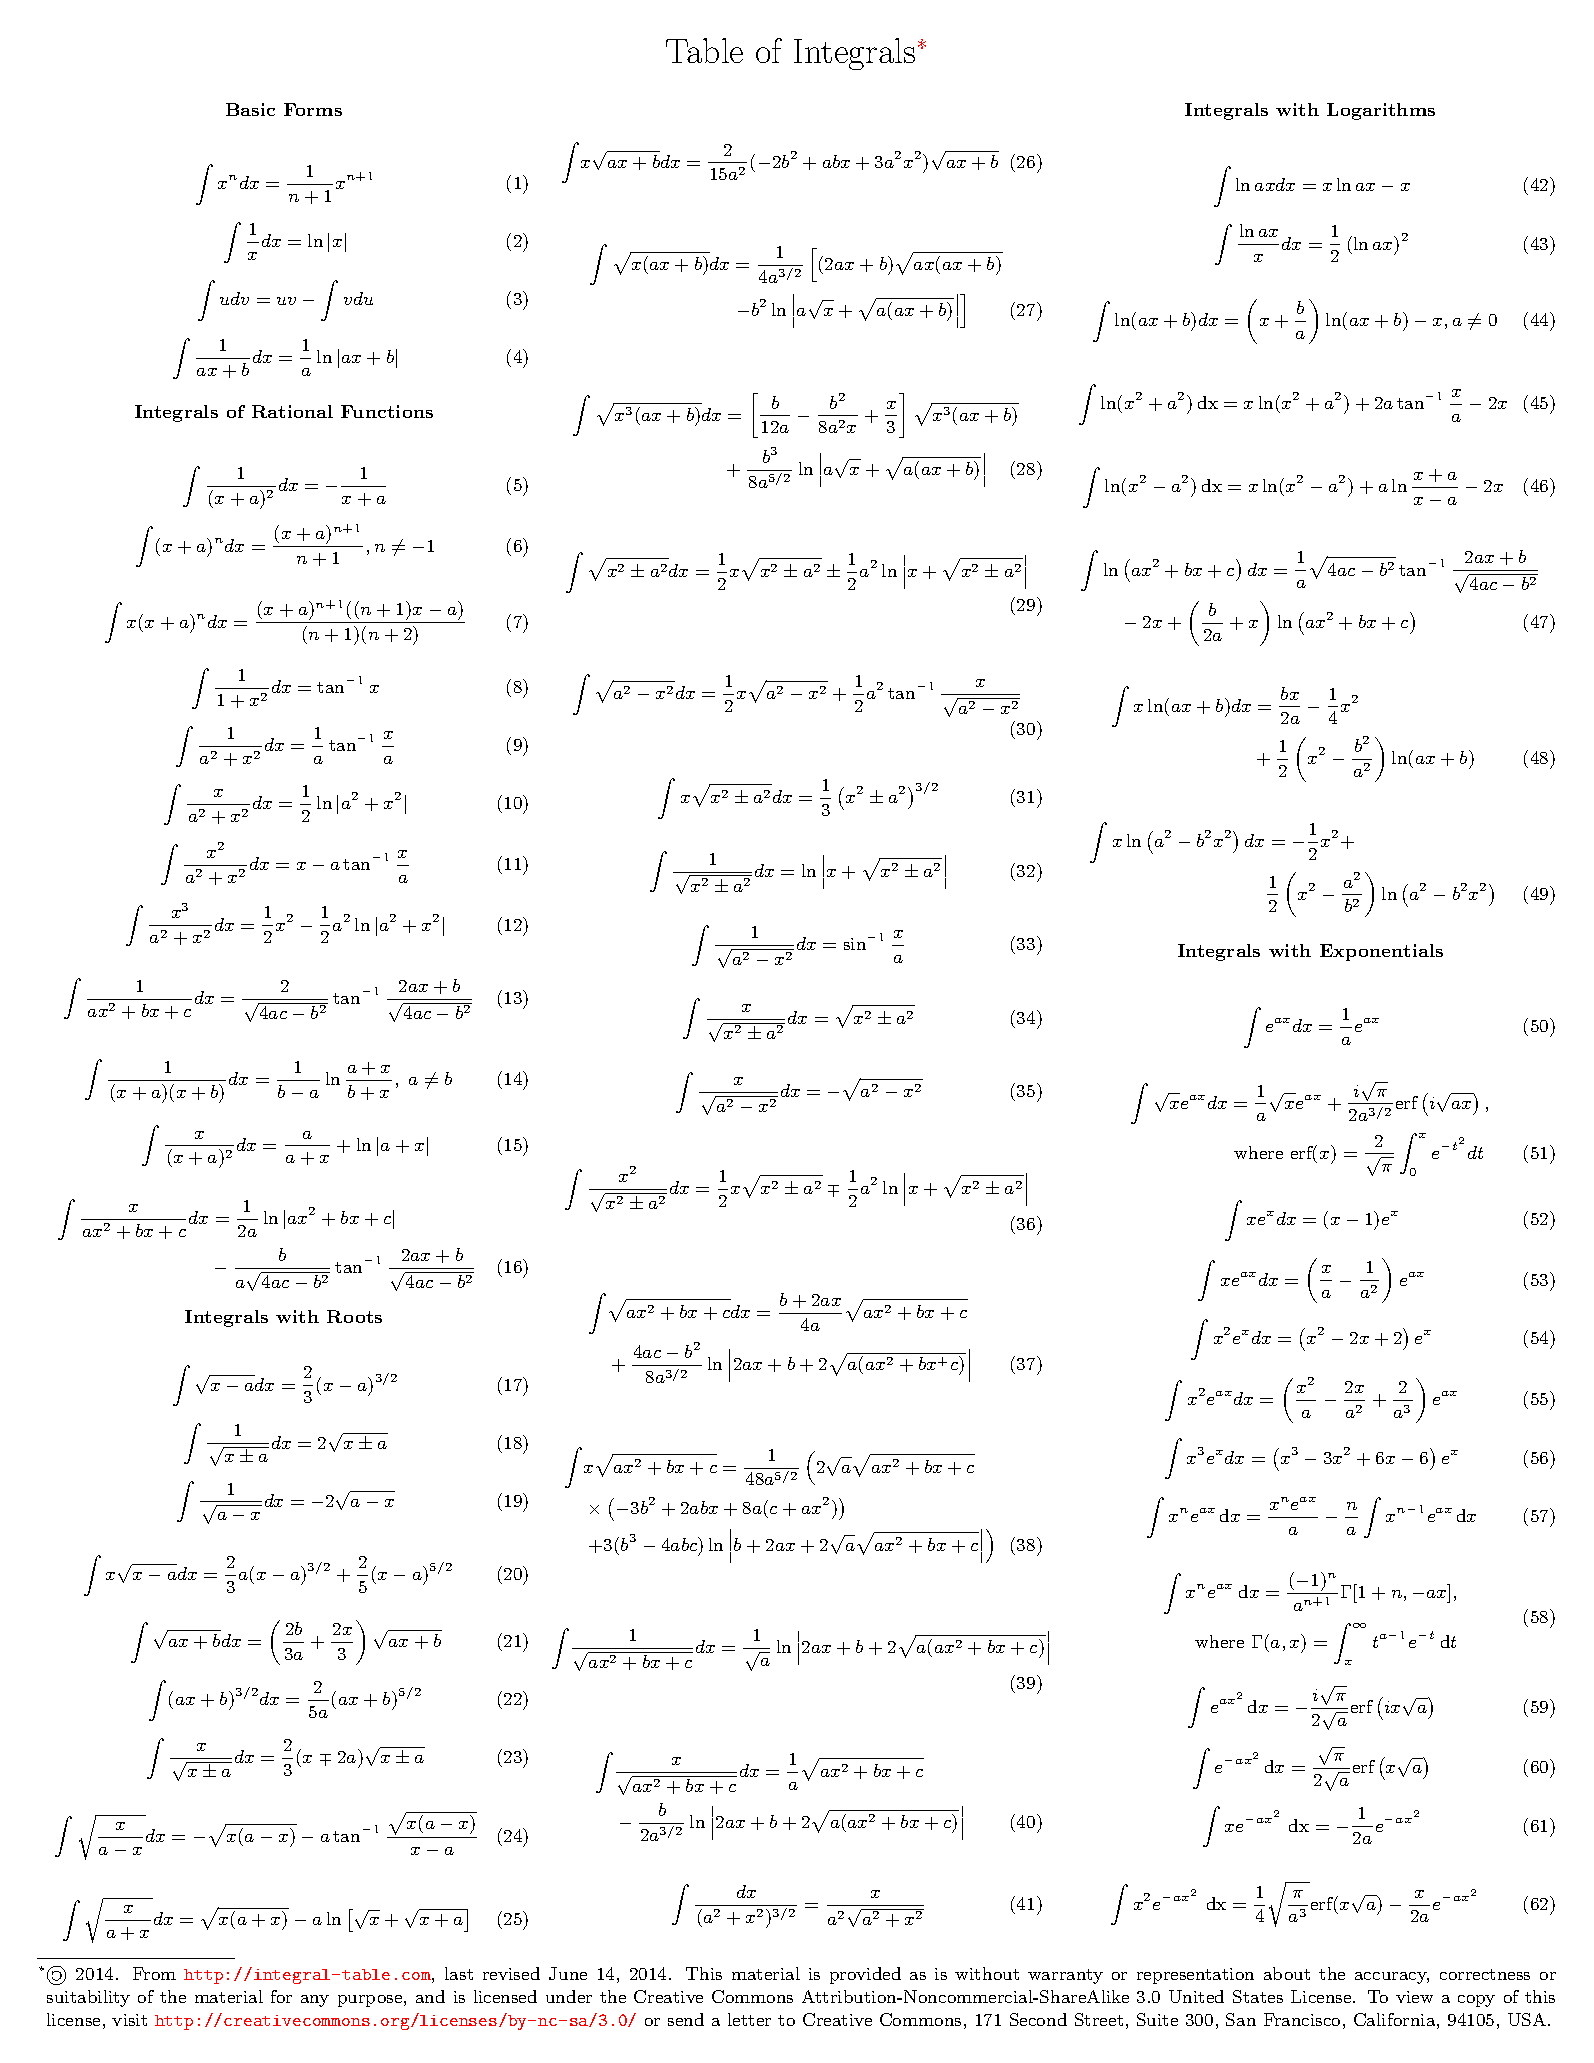
\includepdf[pages={1, 2}, pagecommand={\pagestyle{fancy}}]{integral-table}

\end{document}
